%
% The first command in your LaTeX source must be the \documentclass command.
\documentclass[sigconf]{acmart}

%
% defining the \BibTeX command - from Oren Patashnik's original BibTeX documentation.
\def\BibTeX{{\rm B\kern-.05em{\sc i\kern-.025em b}\kern-.08emT\kern-.1667em\lower.7ex\hbox{E}\kern-.125emX}}

% Rights management information.
% This information is sent to you when you complete the rights form.
% These commands have SAMPLE values in them; it is your responsibility as an author to replace
% the commands and values with those provided to you when you complete the rights form.
%
% These commands are for a PROCEEDINGS abstract or paper.
% \copyrightyear{2019}
% \acmYear{2019}
% \setcopyright{acmlicensed}
% \acmConference[DEBS '19]{DEBS '19: ACM International Conference on Distributed and Event-Based Systems.}{June 24--28, 2019}{Darmstadt, Darmstadt}
% \acmBooktitle{DEBS '19: ACM International Conference on Distributed and Event-Based Systems, June 24--28, 2019, Darmstadt, Darmstadt}
% \acmPrice{15.00}
% \acmDOI{10.1145/1122445.1122456}
% \acmISBN{978-1-4503-9999-9/18/06}

%
% These commands are for a JOURNAL article.
%\setcopyright{acmcopyright}
%\acmJournal{TOG}
%\acmYear{2018}\acmVolume{37}\acmNumber{4}\acmArticle{111}\acmMonth{8}
%\acmDOI{10.1145/1122445.1122456}

%
% Submission ID.
% Use this when submitting an article to a sponsored event. You'll receive a unique submission ID from the organizers
% of the event, and this ID should be used as the parameter to this command.
%\acmSubmissionID{123-A56-BU3}

%
% The majority of ACM publications use numbered citations and references. If you are preparing content for an event
% sponsored by ACM SIGGRAPH, you must use the "author-year" style of citations and references. Uncommenting
% the next command will enable that style.
%\citestyle{acmauthoryear}





% HERE STARTS OUR packages

% \usepackage{balance}  % for  \balance command ON LAST PAGE  (only there!)

% \usepackage{multirow}
% \usepackage [table]{xcolor}

% \usepackage{graphicx}
% \usepackage{color}
% \usepackage{times}
%\usepackage{url}
%\usepackage[utf8]{inputenc}
%\usepackage{soul}
%\usepackage{nameref}
%\usepackage{amsbsy}
% \usepackage{bezier}
% \usepackage{colortbl}
% \usepackage{verbatim}
%\usepackage{qtree}
% \usepackage{xcolor}
% \usepackage{xspace}
% \usepackage{rotating}
% \usepackage{multirow}
%\usepackage{hyperref}
%\usepackage[capitalize]{cleveref}
% \usepackage{todonotes}
% \usepackage{microtype}
% \usepackage{fmtcount}
% \usepackage{datetime}
%\usepackage{tikz}
% \usepackage{pgfplots}
% \usepackage{tcolorbox}
% \usepackage{subfig}
%\usepackage{fancyvrb}

%\usepackage{fancyvrb}
% \usepackage{float}
%\usepackage{mathpazo}
% \usepackage[boxruled,slide,lined]{algorithm2e}

%\usepackage{caption}
% \usepackage{graphicx}
% \usepackage{subcaption}
% \usepackage{graphicx}
%\usepackage{courier}
% \usepackage{cleveref}
% \usepackage{amsmath}
% \usepackage{amssymb}
% \usepackage{latexsym}
% \usepackage{bm}
% \usepackage{subscript}
% \usepackage{multirow}
%\usepackage{tgheros}
% \usepackage{hyperref}
% \usepackage{subfig}

% \usepackage{listings}
%
% \lstset{
% language=Java,                  % the language of the code
% basicstyle=\scriptsize,        % the size of the fonts that are used for the code
% basicstyle=\ttfamily,           % the font used for the code
% backgroundcolor=\color{white},  % choose the background color. You must add \usepackage{color}
% showspaces=false,               % show spaces adding particular underscores
% showstringspaces=false,         % underline spaces within strings
% showtabs=false,                 % show tabs within strings adding particular underscores
% frame=none,                     % adds a frame around the code, none, single
% tabsize=1,                       % sets default tabsize to 2 spaces
% captionpos=b,                      % sets the caption-position to bottom
% breaklines=flase,                % sets automatic line breaking
% % breakatwhitespace=false,      % sets if automatic breaks should only happen at whitespace
% title=\lstname,                 % show the filename of files included with \lstinputlisting;
%                                 % also try caption instead of title
% escapeinside={\%*}{*)},         % if you want to add a comment within your code
% morekeywords={*,...},            % if you want to add more keywords to the set
% belowcaptionskip=-1.6em,
% belowskip=0em,
% framexleftmargin=10pt
% }
%
%
%
% \newcommand{\TODO}[1]{\todo[inline,color=orange!40]{KIA: #1}}


%
% end of the preamble, start of the body of the document source.
\begin{document}

%
% The "title" command has an optional parameter, allowing the author to define a "short title" to be used in page headers.
% \title{Grand Challenge: A Real-Time Multi-class Classifier for High-Speed Streaming Data}

\title{Grand Challenge: Real-Time Object Recognition from Streaming LiDAR Point Cloud Data}


%
% The "author" command and its associated commands are used to define the authors and their affiliations.
% Of note is the shared affiliation of the first two authors, and the "author note" and "author note mark" commands
% used to denote shared contribution to the research.


\author{Sambasiva Rao Gangineni}
\affiliation{%
  \institution{Boston University}
}
\email{samba693@bu.edu}

\author{Harshad Reddy Nalla}
\affiliation{%
    \institution{Boston University}
}
\email{harshad@bu.edu}

% \author{Dimitrije Jankov}
% \affiliation{%
%     \institution{Rice University}
% }
% \email{dimitrijejankov@gmail.com}

\author{Saeed Fathollahzadeh}
\affiliation{%
    \institution{Iran University of Science and Technology}
}
\email{fathollahzadeh@comp.iust.ac.ir}

\author{Kia Teymourian}
\affiliation{%
  \institution{Boston University}
 }
\email{kiat@bu.edu}



%
% By default, the full list of authors will be used in the page headers. Often, this list is too long and will overlap
% other information printed in the page headers. This command allows the author to define a more concise list
% of authors' names for this purpose.
\renewcommand{\shortauthors}{Gangineni, et al.}

%
% The abstract is a short summary of the work to be presented in the article.
\begin{abstract}
% Recognition of objects surrounding a robot in a dynamic environment is one of the research challenges in robotics.
In many robotic applications, LiDAR (Light Detection and Ranging) scanner is used to gather data about the environment.
Applications like autonomous vehicles require real-time processing of LiDAR point cloud data with high accuracy.

We describe in this paper, our implementation for DEBS 2019 Grand Challenge for an object recognition system from high-speed
LiDAR data stream. Our system includes a data processing pipeline with 3 main stages, 
1. LiDAR data filtering 2. Object segmentation and noise reduction 3. Multi-class object classification using Convolutional Neural Network (CNN). 
% We have evaluated our system using point cloud data in 3D and in the projection of it into 2D. 
Our evaluation shows that we can classify objects with high accuracy using the point cloud data and neural network. 
However, we observed that the classification may fail if the object segmentation is not separating objects correctly in different segments especially when the objects are largely covering each other. 
We proposed a pre-processing approach for object segmentation based on separating LiDAR data into multiple area sectors before segmenting the objects. 
\end{abstract}


\copyrightyear{2019} 
\acmYear{2019} 
\setcopyright{acmlicensed}
\acmConference[DEBS '19]{DEBS '19: The 13th ACM International Conference on Distributed and Event-based Systems}{June 24--28, 2019}{Darmstadt, Germany}
\acmBooktitle{DEBS '19: The 13th ACM International Conference on Distributed and Event-based Systems (DEBS '19), June 24--28, 2019, Darmstadt, Germany}
\acmPrice{15.00}
\acmDOI{10.1145/3328905.3330297}
\acmISBN{978-1-4503-6794-3/19/06}

\maketitle

\section{Introduction}
% One of the special and still not completely solved problems in robotics research is the real-time object recognition surrounding an autonomous robot.
% Highly dynamic and rapidly changing environment of a robot requires a fast and intelligent system to detect its surrounding objects. 
% Examples of such applications are autonomous vehicles or autonomous cleaning robots that require object recognition in real-time with high accuracy.
% For such applications, it is important to detect surrounding objects accurately in real-time and be able to react proactively based on object classification results.

One of the surveying methods that are used in such an application is a LiDAR scanner (Light Detection and Ranging). A LiDAR laser scanner is used to generate a three-dimensional representation of the surrounding environment. It uses multiple lasers to generate a point cloud of coordinates (x,y,z) of objects in the cartesian coordinate system. LiDAR point cloud data contains information that can be processed to recognize objects. This task requires real-time data processing and an accurate data model to learn and classify different object types.

The ACM DEBS 2019 grand challenge \cite{DEBSGC2019} specifies an object recognition development challenge for LiDAR streaming point cloud data.
The organizers provide a training set of LiDAR data for 28 different object types like the car (2 different types), pedestrian, trees (2 different types),
 ATM machine, pedestrian, benches, container. The DEBS 2019 challenge scenario, data set and evaluation criteria are 
 described by organizers Bodunov et al. in \cite{DEBSGC2019}.

In this paper we describe our implementation for the grand challenge, our contributions are:


\begin{enumerate}
  
  \item Description of our data analysis architecture and processing pipeline including data pre-processing for LiDAR ground removal, 
  data segmentation (generating voxels containing objects ), and multi-class object classification  (Sec.  \ref{sec:Architecture}).
  \item Experimental evaluation and comparisons of different data processing architectures, different data models to achieve high 
  accuracy and real-time data processing (Sec. \ref{sec:Evaluation}).
  \item A brief state-of-the-art study reviewing most related object recognition from LiDAR point cloud.  (Sec. \ref{sec:relatedWork})
  \item A discussion about lessons learned and challenges (Sec. \ref{sec:conclusion} ).
  % \item Future extensions of our implementation
\end{enumerate}










\section{Data Set}
DEBS 2019  Challenge provides a training and test data sets \cite{DEBSGC2019}. 
The data set consist of LiDAR sensor point cloud which has 64 lasers. Each scene includes 72,000 data readings which includes  X, Y, and Z coordinates (Y axis is the shown to be the elevation). 
In each scene objects are placed around the LiDAR scanner and data is collected, example objects are \textbf{ATM machine}, \textbf{pedestrian}, \textbf{benches}, \textbf{cloth recycling container}. 

We build multiple 2D and 3D visualizations of the data like shown in Figures \ref{fig:ground_before},  \ref{fig:after} and \ref{fig:ClusteringWithNoiseFiltering}. 
We also created animated images of the sequences of scenes to see if the sequence of scenes have any relations to each other. 
We observed that sequence of scenes have no relations and scenes are randomly selected from a set of scenes. 
However, in applications like autonomous vehicles, sequences of scenes have a correlations so 
that one can track the object coming in range of LiDAR laser and going out of the range. 
This information could be used to improved the classification accuracy such application.    


% SAEED
% The data provided for the challenge consists of point cloud readings simulated for a LiDAR sensor that mounts 64 lasers Fig.\ref{fig:data_overview} a , each shoot 1125 times per rotation. That is, each scene consists of 72,000 readings. Each reading is composed of attributes where X, Y, and Z coordinates are as presented in Fig.\ref{fig:data_overview} b.
% 
% In each scene, objects are representative of urban environments and are of the following types: \textbf{ATM machine}, \textbf{pedestrian}, \textbf{benches}, \textbf{cloth recycling container}, \textbf{drinking fountain}, \textbf{electrical cabinet}, \textbf{emergency phone}, \textbf{fire hydrant}, \textbf{glass recycling container}, \textbf{ice freeze container}, \textbf{mailbox}, \textbf{trash bins}, \textbf{phone booth}, \textbf{trees}, and \textbf{several vehicle types}. In some cases, it is possible for an object in a scene to be hidden from the LiDAR sensor (e.g., when such object is occluded by other objects in the scene)\cite{DEBSGC2019}.


% 
% \begin{figure*}[!ht]
% \begin{center}
%   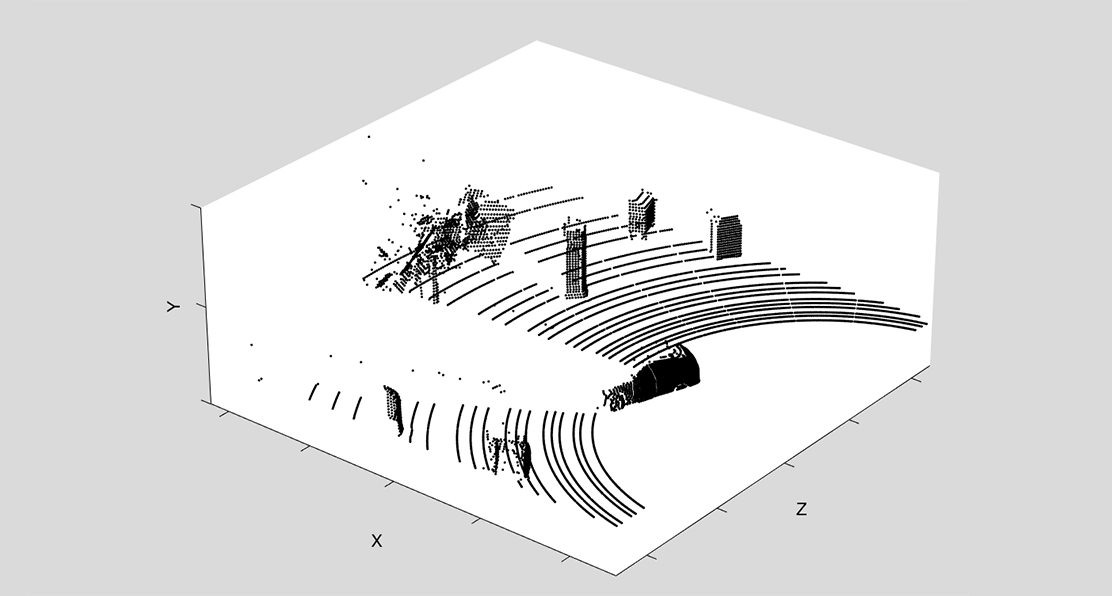
\includegraphics[width=0.8\textwidth]{./images/GC1.png}
%   \caption{An Overview of Data Set from Point Cloud of a single Scene}
%   \label{fig:data_overview}
% \end{center}
% \end{figure*}

%\usepackage{graphics} is needed for \includegraphics


% \begin{figure}%
% 	\centering
% 	\subfloat[point cloud readings simulated for a LiDAR sensor]{{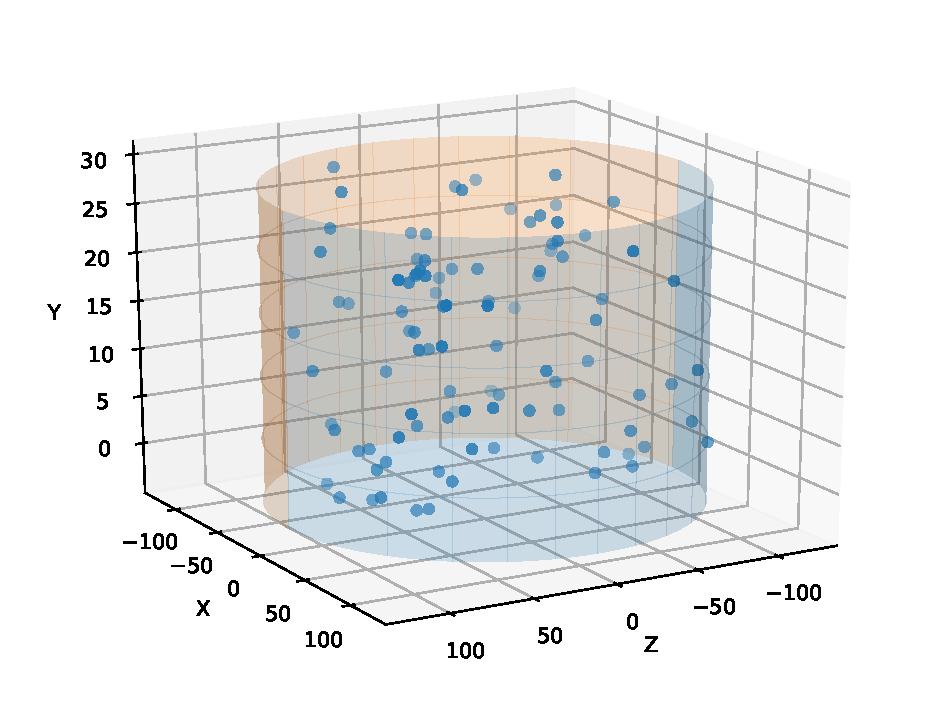
\includegraphics[width=7cm]{images/data_overview.pdf} }}%
% 	\qquad
% 	\subfloat[a scene with different numbers of objects]{{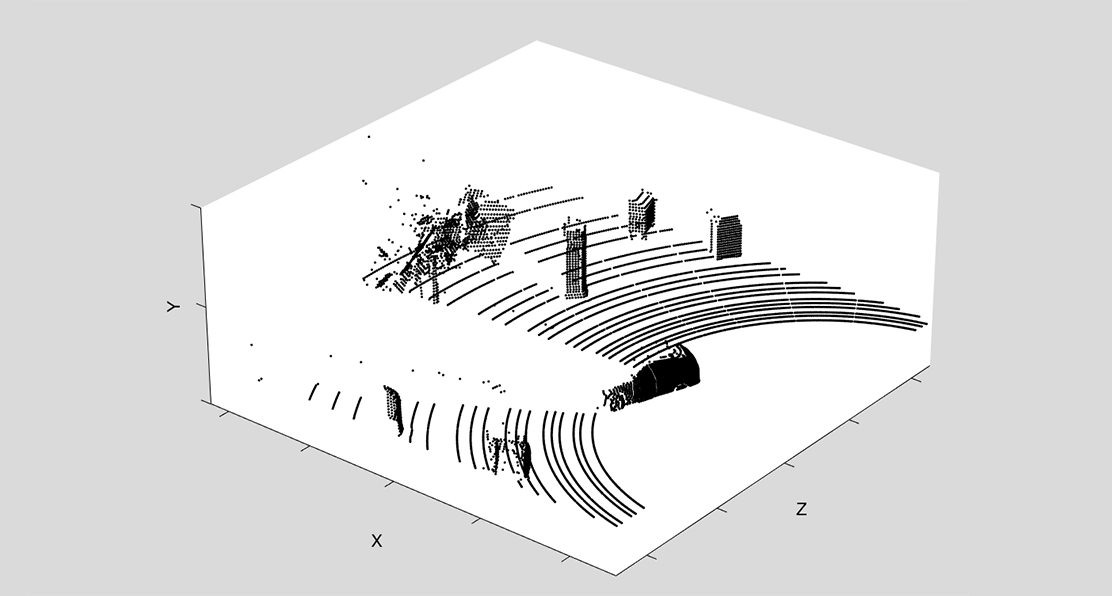
\includegraphics[width=5cm]{images/GC1.png} }}%
% 	\caption{An Overview of Data Set from Point Cloud of a single Scene}%
% 	\label{fig:data_overview}%
% \end{figure}


%KIA 
%Briefly describe the data set and cite the main grand challange paper. 

%We just need to describe what the data is about. 

% We need to mention other data sets like The KITTI Dataset \cite{Geiger2013IJRR}


% KITTI Dataset \cite{Geiger2013IJRR}

\section{Architecture}\label{sec:Architecture}




% Describe the data processing pipeline here. 


% 1. Get the raw data and remove the ground (LiDAR data clean up)
% 2. Segment data and sent it to classifier 
% 3. Classification with Neural Network. 


Figure \ref{fig:dataPipeline} depicts  

\begin{figure*}[h!]
 \begin{center}
   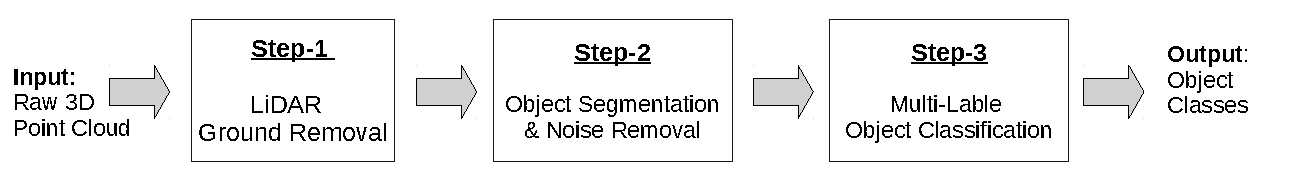
\includegraphics[width=0.9\textwidth]{./images/DataProcessingPipleline.pdf}
   \caption{An Overview of our Data Processing Architecture}
   \label{fig:dataPipeline}
 \end{center}
\end{figure*}





Describe \ldots. 

Different forms of data processing architectures that we have implemented and tested . 

\begin{enumerate}
  \item Different methods for removing noise from raw data (data preprocessing). 
  \item Projecting 3D data into 2D data using 3 different projection methods 
  \item CNN  (with and without maxpool) + fully-connected + dropout + fully-connected+softmax
  \item CNN with different number of hidden layers. 

\end{enumerate}



% KIA
% We need another image to describe the CNN architecture. 
% Add two images about it. 





\subsection{Multi-class Object Classification}
% Describe here the CNN architecture.
We use for classification of point cloud data Convolutional Neural Network (CNN).
Our neural network architecture is represented in Figure \ref{fig:cnn}.
The network model is designed for multi-class classification of 
point cloud objects.
% Convolutional neural network provides a promising result of object model with spatial data.
CNN effectively learns the feature recognition of planes, corners, and the edges of the object model.
Our network model is designed with 4 convolutional layers where each layer filter is expected to
recognize planes, corners, edges, and distribution of the objects per orientation.
Other layers learn the global label for the input grid from the knowledge passed by each layer.

\textbf{Input preparation:}
The 3D points \textit{(x,y,z)} of the object are projected into 2D points \textit{(x,y) or (x',y')} (Sec 3.2).
These projected object points are placed on a grid of height 7 and length 10.
This grid is divided into cells of 0.1x0.1 resulting in 70x100 cells and the information about the number of points in each cell is the input to the model.
This input on plotting as pixels will result in the object.

\textbf{Input layer:}
The network model takes a fixed-size input of NxM point counts in grid-cells. We have
used $N=70$ and $M=100$ for our model requirements. The input layer forwards each object input to the 1st layer
of convolutional.


\textbf{Convolutional Layer (input,f,s):}
There are 4 convolutional layers in our architecture to learn features on each orientation.
The first convolutional layer feed on two-dimensional input of size $N \times  M$ from
the input layer, a filter size=f and number of filters=s to be applied.

The filter-size provided to convolutional layer is $5 \times 5$ with 16 such filters to be applied on the input.
The convolutional layer uses filter f to apply convolution operation on input to create a feature map as output.
The convolutional layer learns about the spatial planes, edges, and distribution in the object,
the convolutional layer passes the output to the rectified linear unit (ReLU) before feeding
it forwards to next layers.

\textbf{Max Pooling layer:}
The pooling layer is added to reduce the dimension of the data by a factor of d. 
The size of pooling layer is  $d \times  d$, in our model d = 2. 
The max pooling layer is applied after each alternative convolutional
layer, it reduces the dimension of the feature map with their maximums.

\textbf{Dropout Layer:}
Dropout layer is used for reducing overfitting. As the network is executed on the iterative model with a feed forward network.
The model network tends to overfit on the data. Dropout layer drops random samples from the feature
map while training.

\textbf{Fully Connected Layer:}
As fully connected layers contain n output neurons. Each neuron of the output is a learned linear
combination of all the outputs from the previous layer, passed through a nonlinearity.
We use ReLUs to save the final output layer, where the number of outputs corresponds
to the number of class labels and a softmax nonlinearity is used to provide a probabilistic output.


% Our Network model starts with an input layer feeding to convolution layer with ReLu then
% another convolutional layer with ReLu and max pool layer then passing input to another batch of convolutional layers
% with Relu and convolutional layer with Relu and max pool, then the feature map is flattened to be feed-forwarded to
% fully connected layer with ReLu, then random samples are dropped with dropout layers
% and finally fed to a fully connected layer and softmax to classify the object into multiclass.

The combination of the above layers is used by some of the state-of-the-art models which have high accuracy on 2-D image inputs.
In order to build the model for this challenge, we have used the above layers, because the input to the model is in the form of pixels.
% Different configurations had different resulted in different models.
%To come up with the state-of-the-art architecture,

\textbf{Model:}
Single objects data is used as input for training the model. We started with implementing a simple 2 layered convolutional neural network,
which uses two convolutional layers with rectified linear unit and a max pool layer,
drop out and a couple of fully connected layers to classify point cloud objects based upon classes.
This architecture was effective but 
did not give acceptable results. 
%%%%%decide%%%%%% the test accuracy on single objects is low
Further experimenting with layers explained the learning of pixel input by convolutional layer.

The experiment with 4 layered convolutional network has better performance, as they were able to learn planes, edges, and distribution of the point cloud object.
A couple of 2 convolutional layers with alternative Relu added before output and max-pooling layer between them shows the best results while training and testing on individual objects.

The architecture was added with 2 fully connected layers with a single drop out layer to reduce overfitting.
This experimented architecture showed the best result with the training set and the evaluation platform.

\begin{figure*}[!h]
     \begin{center}
       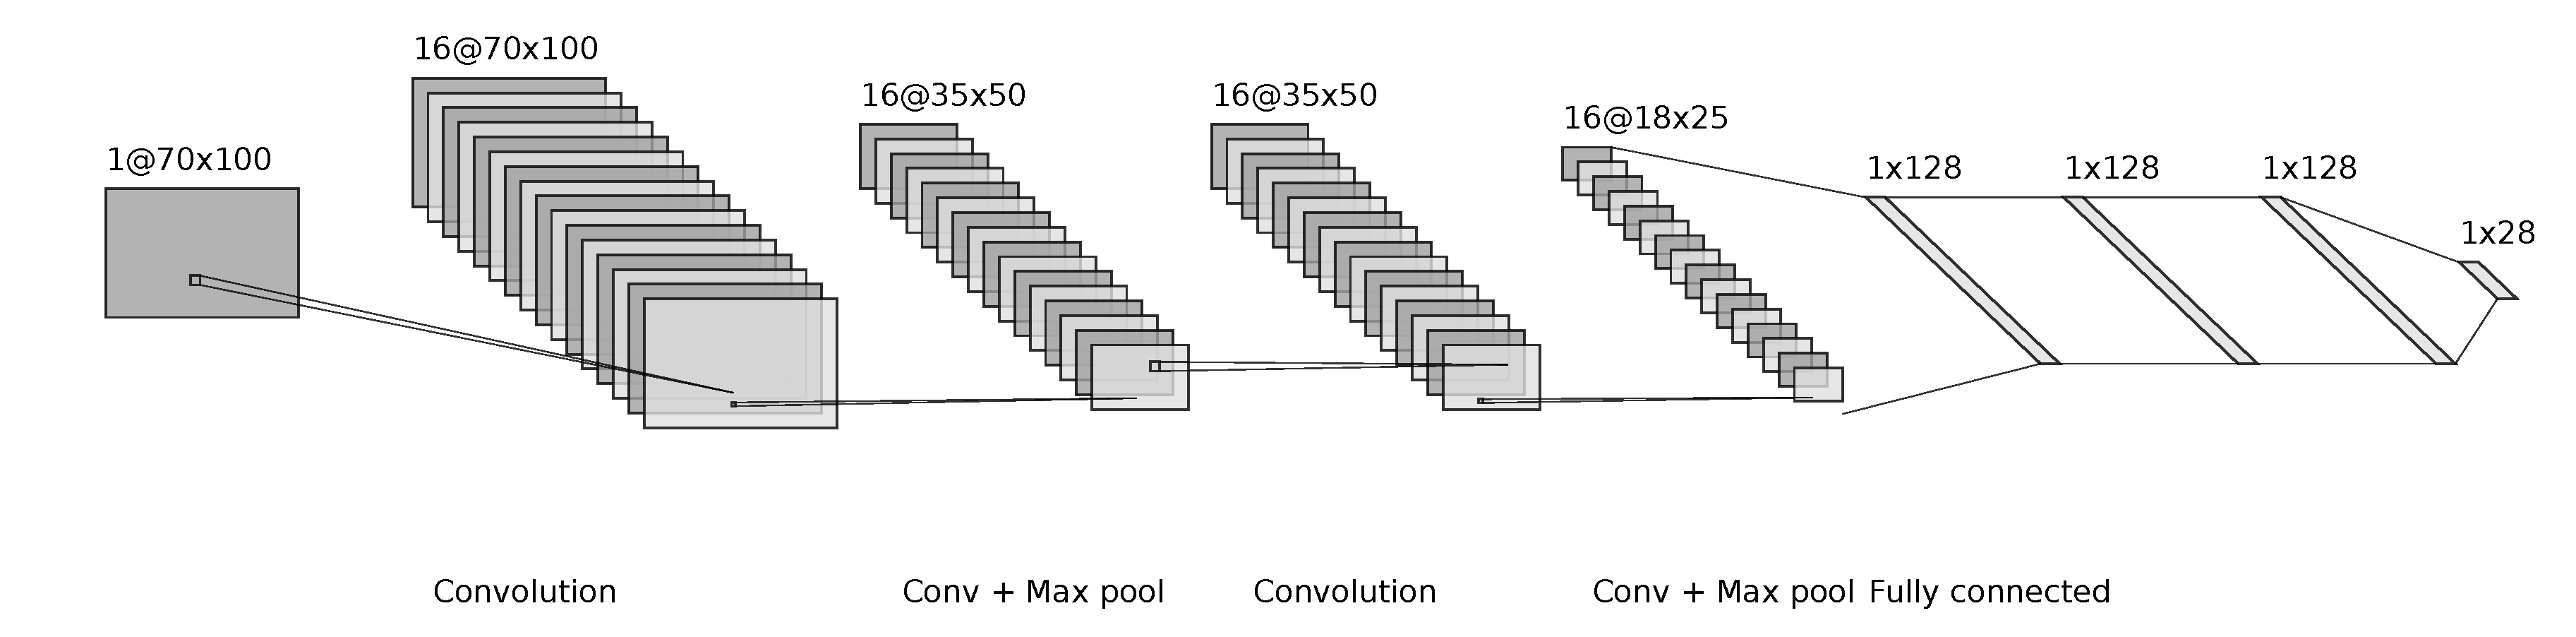
\includegraphics[width=0.8\textwidth]{./images/object_net.pdf}
       \caption{Overview of Convolutional Neural Network Layers with 4 Convolutional Layers}
       \label{fig:cnn}
     \end{center}
\end{figure*}

\subsection{CNN with 3D point cloud Input Data}
We experimented with 3D CNN as dataset could be transformed into the input of 3D CNN being a 3D point cloud dataset.
Our approach was to convert point clouds into a set of voxels by voxelization. Voxelization is the process of conversion of a geometric object from its continuous geometric representation into a set of voxels that best approximates the continuous
object. We used the process to fit a bounding box voxel around the point cloud to form a voxel grid.

We designed for 4 layered 3D CNN architecture with 2 fully connected layers, a dropout layer, around a softmax layer at the end.
The voxel-grid is feed into the network as input and network predict the object out the 28 classes on which network is trained.
The 3D CNN model gave the best performance when trained on a minimal number of class attributes but failed to perform when trained on all the class.
The major reason we tracked for low performance of 3D CNN with a large number of output classes was the density of the object and its distribution.

The performance could be improved by experimenting with lower voxel size to increase more voxels for input.
This method is high resources dependent as the input size grows from several megabytes to several gigabytes, making harder to work on a standard system.
Reviewing the performance between 2D CNN and 3D CNN, the 2D CNN model was providing better performance and precision.



\section{Evaluation}\label{sec:Evaluation}

\TODO{Describe the evaluation set up briefly.}



\TODO{- 3 Graph that compares the prcision/recall (F1) and time perofrmance of our multiple approaches. 
}


\TODO{Our appriaches are: 
1. Graphs for 2D CNN with simple linear projection on one of the axis.
2. 2D CNN with improved transformation from 3D to 2D CNN
3. 2D CNN - with - separation and projection and then segmentation with DBSCAN 
4. 3D CNN
5. Different No. of Layers up to 3 and 2 different size of filter. 
 }


- We should run it on a standard machine (better on EC2 because it is better reproducable) and show the processong time performance. 


- We present on our plots, Precision/Recall and Processing time. 






\section{Related Work}\label{sec:relatedWork}
In this brief section, we review some of the most related publications regarding LiDAR point cloud object recognition problem.

%SAEED: describe some related work:
\textbf{3D shape analysis} Performance of 3D shape analysis is heavily dependent on the input representation. 
The main representations are volumetric, point cloud and multi-view.

To better compare 3D shape descriptors, we will focus on retrieval performance. Recent
approaches show significant improvements in retrieval. Yavartanoo et al. \cite{DBLP:journals/corr/abs-1811-01571} 
introduces multi-view stereographic projection; it first transforms a 3D input volume into a 2D planar image using stereographic projection.

Zhou et al. \cite{Zhou_2018_CVPR} proposed a model that operates only on LiDAR data. 
In regard to that, it is the best-ranked model on KITTI \cite{geiger2012we} for 3D and birds-eye view detections using LiDAR data only. 
The basic idea is end-to-end learning that operates on grid cells without using handcrafted features. However, even with sparse 3D convolution 
operations, this model's computational speed is still slower than other similar proposed architectures.


Wu et al. \cite{DBLP:conf/icra/WuWYK18} present SqueezeSeg which projects point cloud to the front view with cells gridded by LiDAR rotation. 
It applies normal 2D CNN for classification and segmentation. The front view representation of point cloud shares 
the same multi-scale problem like the camera because the sizes of objects change as the distance varies.

Riegler et al \cite{DBLP:conf/cvpr/RieglerUG17} design more efficient 3D CNN or neural network architectures that exploit sparsity in the point cloud. 
However, these CNN based methods still require quantization of point clouds with certain voxel resolution.

Huang et al. \cite{DBLP:conf/icpr/HuangY16} take a point cloud and parse it through a dense voxel grid, generating a set of occupancy voxels which are used as input to a 3D CNN to produce one label per voxel. They map back the labels to the point cloud. Although this approach has been applied successfully, it has disadvantages like quantization, loss of spatial information, and unnecessarily large representations.

Maturana et al. \cite{DBLP:conf/iros/MaturanaS15} used deep learning models is to first convert raw point cloud data into a 
volumetric representation, namely a 3D grid. This approach, however, usually introduces quantization artifacts and excessive memory usage, making it difficult to go to capture high-resolution or fine-grained features.


The defined grand challenge 2019 \cite{DEBSGC2019} scenario for an object is slightly different from
the above described state-of-the-art because of the following reasons: (i) We need to classify and
count the objects and this is different than semantic segmentation of point clouds. (ii) Objects
can partially cover each other and it is required to classify them with counts of objects.   
(iii) Scenes have no relations and are random selected. 




% KIA: I just put the paper titles here \ldots
% Yavartanoo et al. \cite{DBLP:journals/corr/abs-1811-01571} propose an approach for 3D object classification  named SPNet - it is a deep 3D object classification and retrieval using stereographic projection.

%Wu et al. \cite{DBLP:conf/icra/WuWYK18} propose an approach for 3D LiDAR segmentation. SqueezeSeg: Convolutional Neural Nets with Recurrent {CRF} for Real-Time Road-Object Segmentation from 3D LiDAR Point Cloud.

%Yin et al. \cite{Zhou_2018_CVPR}  VoxelNet: End-to-End Learning for Point Cloud-Based 3D Object Detection.

%Riegler et al \cite{DBLP:conf/cvpr/RieglerUG17} OctNet: Learning Deep 3D Representations at High Resolutions.

%Huang et al. \cite{DBLP:conf/icpr/HuangY16}  Point cloud labeling using a 3D convolutional neural network.


%Maturana et al. \cite{DBLP:conf/iros/MaturanaS15}  VoxNet: {A} 3D convolutional neural network for real-time object recognition.



\section{Conclusion and Future Work}\label{sec:conclusion}













\bibliographystyle{ACM-Reference-Format}
\bibliography{refrences}




\end{document}
